\documentclass[12pt,a4paper]{article}
\usepackage{amsmath,amssymb,amsthm,bm}
\usepackage{geometry}
\geometry{margin=2.5cm}
\usepackage{hyperref}
\usepackage{booktabs}
\usepackage{array}
\usepackage{xcolor}
\usepackage{graphicx}
\usepackage{longtable}

\newcommand{\CMSTG}{\textsc{cmstg}}
\newcommand{\Psibar}{\bar\Psi}
\newcommand{\Feff}{F_{\rm eff}}
\newcommand{\Lbare}{\Lambda_{\rm bare}}
\newcommand{\Lz}{\Lambda_0}
\newcommand{\Mpl}{M_{\rm Pl}}
\newcommand{\thetastar}{\theta_*}
\newcommand{\rs}{r_s}
\newcommand{\DC}{D_C^*}

\theoremstyle{plain}
\newtheorem{theorem}{Theorem}

\title{\textbf{Two Structural No-Go Theorems for Late-Time Modifications\\
       of Dark Energy in Curvature-Memory Scalar-Tensor Gravity}}
\author{Christopher~R.~B.~Wilson\thanks{Email: \texttt{C.Isomorph@gmail.com}. Independent researcher.}}
\date{2026}

\begin{document}
\maketitle

\begin{abstract}
This is Paper~I of a four-paper series on Curvature-Memory Scalar-Tensor
Gravity (\CMSTG), a covariant scalar-tensor extension of general relativity
in which a scalar field $\Psi$ encodes retarded curvature history through a
non-minimal coupling $\Lz\Psi^2 R$ to the Ricci scalar. The framework,
developed in detail in Paper~II, passes all current precision cosmological
tests with one residual: a $2.77\sigma$ tension with DESI~Y1 BAO data.
This paper establishes that the residual is structural --- irreducible within
the \CMSTG\ action class --- by proving two complementary no-go theorems.
Together they prove the Phase~1 canonical action is the unique covariant
scalar-tensor solution within its action class consistent with both Planck
CMB data and DESI~Y1 BAO data simultaneously.
\textbf{Theorem~1}: any scalar field sourced by the Ricci scalar $R>0$
and initialized at zero grows monotonically, increasing the effective
gravitational coupling $\Feff$ and suppressing $H(z)$ at DESI
redshifts---the wrong direction to reduce the $2.77\sigma$ DESI~Y1
tension. \textbf{Theorem~2}: any mechanism that raises $H(z)$ in the
interval $z\in[0,z_{\rm rec}]$ while keeping the sound horizon $\rs$
fixed necessarily shifts the CMB acoustic angle $\thetastar$ above the
Planck bound at more than $30\sigma$. Fourteen simulation-based mechanism
tests (SIM131--SIM136, SIM141--SIM144, plus two structural arguments)
verify both theorems exhaustively across the identified Tier~2 mechanism
space, including a completeness probe (SIM144) confirming that scalars
with simultaneous curvature and matter coupling also fail.
The $2.77\sigma$ DESI~Y1 residual is therefore a structural
prediction of Phase~1 canonical \CMSTG, not a defect in the action; the
decisive test is DESI~Y3.

Companion papers establish (II)~the framework, field equations, and
cosmological consistency of \CMSTG~\cite{WilsonPaperII}; (III)~the UV
finiteness and renormalization-group flow~\cite{WilsonPaperIII}; and
(IV)~galactic-scale constraints establishing the dark-matter boundary of
the theory~\cite{WilsonPaperIV}. This paper establishes the dark-energy
boundary.
\end{abstract}

\noindent\textbf{Keywords:} dark energy theory; modified gravity; CMB; baryon acoustic oscillations; scalar-tensor theories

\tableofcontents
\bigskip

% ─────────────────────────────────────────────────────────────────────────────
\section{Introduction}
\label{sec:intro}

Curvature-Memory Scalar-Tensor Gravity (\CMSTG) is a covariant scalar-tensor
extension of general relativity in which the scalar field $\Psi$ encodes
retarded curvature history through a non-minimal coupling $\Lz\Psi^2 R$. The
framework, its action, and its passing record against precision cosmological
data are developed in detail in Paper~II of this series~\cite{WilsonPaperII}.
The single open question raised by Paper~II is whether the $2.77\sigma$
residual against the DESI~Y1 BAO dataset can be reduced within the \CMSTG\
action class by extending the action, deforming its parameters, or coupling
additional fields. This paper proves that the answer is no: the residual is
structural.

The argument rests on two theorems, each verified by an exhaustive mechanism
scan. The first theorem closes the gravitational-sector route (modifications
acting through $\Feff$); the second closes the energy-density route
(modifications acting through $H(z)$ directly). Together they establish that
the Phase~1 canonical $H(z)$ profile is the unique solution consistent with
Planck CMB and DESI~Y1 BAO simultaneously, within the action class.

The Phase~1 canonical \CMSTG\ action of Paper~II~\cite{WilsonPaperII} is
\begin{equation}
  S_{\rm P1} = \int\!d^4x\,\sqrt{-g}\,\Bigl[
    \tfrac{1+2\Lz\Psi^2}{2}\,R
    - \tfrac{1}{2}(\partial\Psi)^2
  \Bigr] + S_{\rm SM}\,,
  \label{eq:phase1-action}
\end{equation}
with $\Lz = 0.003\,\Mpl^{-2}$, $\Psibar = 2.62\,\Mpl$, and effective
gravitational coupling $\Feff = (1+2\Lz\Psibar^2)/2 = 0.521$, passes all
current precision observational criteria: CMB TT/TE/EE power spectra (Planck
plikHM), BOSS and DESI~Y1 BAO, RSD growth rate $f\sigma_8$, gravitational wave
speed $c_T=c$~\cite{Abbott2017,Creminelli2017}, and Solar System PPN bounds~\cite{Planck2018,BOSS2017,DESI2024}.
It is UV-finite through two loops with an explicit $\Lz$ fixed point at
$\Lz=0$ (Paper~III of this series~\cite{WilsonPaperIII}). Its one
remaining residual is a $2.77\sigma$ tension with the DESI~Y1 BAO dataset
(joint MCMC $\chi^2_{\rm DESI}=18.26$).

Whether this residual is reducible within the \CMSTG\ action class---by
extending, deforming, or coupling additional fields---is the central question
addressed by three successive simulation programmes (Phases 2--4, SIM112--SIM144),
summarised in companion notes available at the repository.
The answer, established here, is no.

This is Paper~I of a four-paper series; companion papers establish
(II)~the framework and observational consistency~\cite{WilsonPaperII},
(III)~the UV structure~\cite{WilsonPaperIII}, and (IV)~galactic-scale
constraints~\cite{WilsonPaperIV}.

The $2.77\sigma$ floor arises from a geometric constraint: with $\Feff > 1/2$,
the effective Newton constant $G_{\rm eff} = G/(2\Feff) < G$, suppressing $H(z)$
relative to $\Lambda$CDM at DESI redshifts $z\in[0.5,\,1.3]$. To reduce the
DESI tension, a modification must either (a) reduce $\Feff$ at intermediate
redshifts relative to the CMB epoch, or (b) add energy density that raises
$H(z)$. We prove that both routes are blocked:
\begin{itemize}
  \item \textbf{Route (a)} requires a curvature-sourced scalar to decrease
        $\Feff$ toward $z=0$. Theorem~1 shows that any such scalar, initialized
        at zero as required by the Deser--Woodard boundary condition, instead
        increases $\Feff$ monotonically---the wrong direction.
  \item \textbf{Route (b)} requires raising $H(z)$ at $z<z_{\rm rec}\approx
        1090$ while preserving CMB observables. Theorem~2 shows this is
        impossible at fixed sound horizon: any late-time $H(z)$ boost shifts
        the CMB acoustic angle $\thetastar$ by tens of $\sigma$ above the
        Planck bound.
\end{itemize}

Together, the two theorems constitute a two-sided no-go for the DESI residual,
with the first eliminating downward mechanisms and the second eliminating upward
mechanisms. The Phase~1 canonical action is the unique attractor consistent
with both datasets.

This paper presents each theorem, its proof, and the full set of mechanism
tests that verify it is exhaustive. Section~\ref{sec:nogo1} covers Theorem~1
and the six Phase~3 probes (SIM131--SIM136). Section~\ref{sec:nogo2} covers
Theorem~2 and the Phase~4 mechanism tests (SIM141--SIM143). Section~\ref{sec:combined}
states the combined no-go structure. Section~\ref{sec:implications} discusses
implications and the DESI~Y3 outlook.

% ─────────────────────────────────────────────────────────────────────────────
\section{Theorem 1: Curvature-Sourced Scalar Extensions}
\label{sec:nogo1}

\subsection{Setup}
\label{sec:nogo1-setup}

The Phase~1 $2.77\sigma$ DESI tension arises because $H(z)$ is systematically
low at $z\in[0.5,1.3]$. The geometric origin is $\Feff = 0.521 > 1/2$:
the effective Newton constant $G_{\rm eff}=G/(2\Feff)$ is weakened, suppressing
expansion. To raise $H(z)$ at DESI redshifts \emph{via the gravitational sector},
one needs $\Feff$ to decrease after recombination---gravity strengthening
toward late times relative to the CMB epoch:
\begin{align}
  \Feff(z_{\rm CMB}) &= 0.521\,, \label{eq:cmc} \\
  \dot\Feff &< 0 \quad\text{after recombination.} \label{eq:desi-req}
\end{align}

A natural candidate is a new scalar field $\phi$ sourced by $R$, motivated by
the Deser--Woodard identification $\Psi=\Box^{-1}R$~\cite{DeserWoodard2007}. The field equation of
motion in FLRW is
\begin{equation}
  \phi'' + (3-\varepsilon_H)\phi' = \xi_\phi \cdot \frac{R}{H^2}
  = 6\xi_\phi(2-\varepsilon_H)\,,
  \label{eq:phi-eom}
\end{equation}
where $N=\ln a$, primes denote $d/dN$, and $\varepsilon_H=-\dot{H}/H^2>0$
during matter domination. The right-hand side is positive throughout cosmic
history for any $\xi_\phi>0$.

\subsection{Theorem Statement and Proof}
\label{sec:nogo1-proof}

\begin{theorem}[First Structural No-Go]
\label{thm:nogo1}
Let $\phi$ be a scalar field satisfying equation~\eqref{eq:phi-eom} with
$\xi_\phi>0$ and initial condition $\phi_{\rm ini}=0$ at $z_{\rm ini}\gg
z_{\rm CMB}$. Then $\phi(z)\geq0$ for all $z\leq z_{\rm ini}$, and any
$\Feff$ that is an increasing function of $\phi$ satisfies $\dot\Feff>0$
after recombination. Conditions~\eqref{eq:cmc} and~\eqref{eq:desi-req}
cannot be simultaneously satisfied.
\end{theorem}

\begin{proof}
Since $R>0$ throughout matter and radiation domination, and $\xi_\phi>0$,
the source term in equation~\eqref{eq:phi-eom} is strictly positive. With
$\phi_{\rm ini}=0$ and $\phi'_{\rm ini}=0$, the solution satisfies $\phi(N)>0$
for all $N>N_{\rm ini}$---the field is driven monotonically positive. For any
$\Feff(\phi)$ with $\partial\Feff/\partial\phi>0$ (e.g.\ $\Feff = F_0 + \xi\phi$
or the quadratic forms tested below), this implies $\dot\Feff>0$. In the
Friedmann equation $H^2 = \rho/(3\Feff)$, a monotonically increasing $\Feff$
suppresses $H(z)$ at late times after self-consistent $\Lbare$ calibration.
Condition~\eqref{eq:desi-req} is violated, and the DESI tension is worsened
rather than reduced. $\square$
\end{proof}

The argument is independent of the functional form of $\Feff(\phi)$: it depends
only on the sign of the curvature source and the zero initial condition. It
also applies to modifications of the $\Psi$ kinetics: any coupling that effectively
adds a positive-definite correction to $\Feff$ from a curvature-sourced field
falls under the same argument.

\subsection{Verification: Six Phase~3 Probes}
\label{sec:nogo1-sims}

Six independent mechanism classes were tested in simulations SIM131--SIM136.
Table~\ref{tab:p3summary} summarises the results.

\begin{table}[h!]
\centering
\caption{Phase~3 simulation summary (SIM131--SIM136). All six probes fail.
Phase~1 canonical reference: DESI $2.77\sigma$, $100\thetastar=1.041$.}
\label{tab:p3summary}
\setlength{\tabcolsep}{5pt}
\begin{tabular}{llcccl}
\toprule
SIM & Mechanism & Tension [$\sigma$] & $100\thetastar$ & $\Delta\chi^2$ & Verdict \\
\midrule
SIM131 & Additive quadratic $+\xi\Psi R$              & 5.97       & 0.797         & $+195$ & FAIL \\
SIM132 & Subtractive quadratic (Deser--Woodard analog) & 3.59--3.83 & 0.922         & $+70$  & FAIL \\
SIM133 & Gauss--Bonnet sourcing                        & 9.68       & $\gg1$        & $+544$ & FAIL \\
SIM134 & Exponential/dilaton coupling                  & 3.59--3.84 & 0.922         & $+70$  & FAIL \\
SIM135 & Bi-scalar ($\Psi$ frozen, $\phi$ sourced)    & 3.73--5.60 & 0.827--0.924  & $+65$--$+170$ & FAIL \\
SIM136 & Horndeski kinetic $G^{\mu\nu}\partial_\mu\Psi\partial_\nu\Psi$ & 3.53--3.75 & 0.870--0.921 & $+56$--$+66$ & FAIL \\
\bottomrule
\end{tabular}
\end{table}

Each probe worsens the DESI tension relative to the Phase~1 canonical
$2.77\sigma$ floor. Two cases deserve comment.

\textit{SIM133 (Gauss--Bonnet):} The Gauss--Bonnet term $\mathcal{G}=R^2-4R_{\mu\nu}R^{\mu\nu}+R_{\mu\nu\rho\sigma}R^{\mu\nu\rho\sigma}$~\cite{Nojiri2005} scales as $\mathcal{G}
\propto H^4$ at $z_{\rm CMB}$, which is $(H/H_0)^2\approx10^6$ larger than
its $z=0$ value. Even the smallest tested coupling $\tilde\alpha=10^{-8}$
drives $\Psi\to -278{,}521\,\Mpl$ before recombination ($\Feff\sim2.3\times10^{8}$,
tension $9.68\sigma$). GB sourcing is CMB-incompatible at any coupling.

\textit{SIM135 (bi-scalar with frozen $\Psi$):} Setting $\Psi$ to its Phase~1
canonical value by construction satisfies $\Feff(z_{\rm CMB})=0.521$
exactly---condition~\eqref{eq:cmc} is met. However, the new field $\phi$,
sourced by $R$ with $\phi_{\rm ini}=0$, still grows monotonically, increasing
$\Feff$ at low redshift and enlarging the angular diameter distance $D_A$.
After self-consistent $\Lbare$ calibration, DESI tension worsens to
$3.73$--$5.60\sigma$.

\textit{SIM136 (Horndeski kinetic):}~\cite{Horndeski1974,Kobayashi2011} At $\Psi_{\rm ini}=0$, the coupling
$\Feff'(0)=2\Lz\times0=0$ provides no sourcing force---$\Psi$ remains zero
throughout. At $\Psi_{\rm ini}=\Psibar$, the scalar is near-frozen
($\Psi'\approx0$) so the Horndeski kinetic contribution
$\alpha H^2\Psi'^2\approx0$: kinetic factor $(1+6\alpha H_0^2)\approx1.003$
across the entire $\alpha$ scan, entirely negligible.

All six probes confirm Theorem~\ref{thm:nogo1}: monotone $\Feff$ growth is
universal across functional forms, coupling structures, and initial conditions
consistent with $\phi_{\rm ini}=0$.

Figure~\ref{fig:psi_evolution} shows the $\phi(z)$ evolution for all six
mechanisms, confirming the monotone growth from zero that drives the no-go.
Figure~\ref{fig:desi_chi2} shows the DESI $\chi^2$ as a function of the
dominant coupling parameter for each mechanism, with the Phase~1 canonical
baseline marked; no curve goes below the baseline.

\begin{figure}[h!]
  \centering
  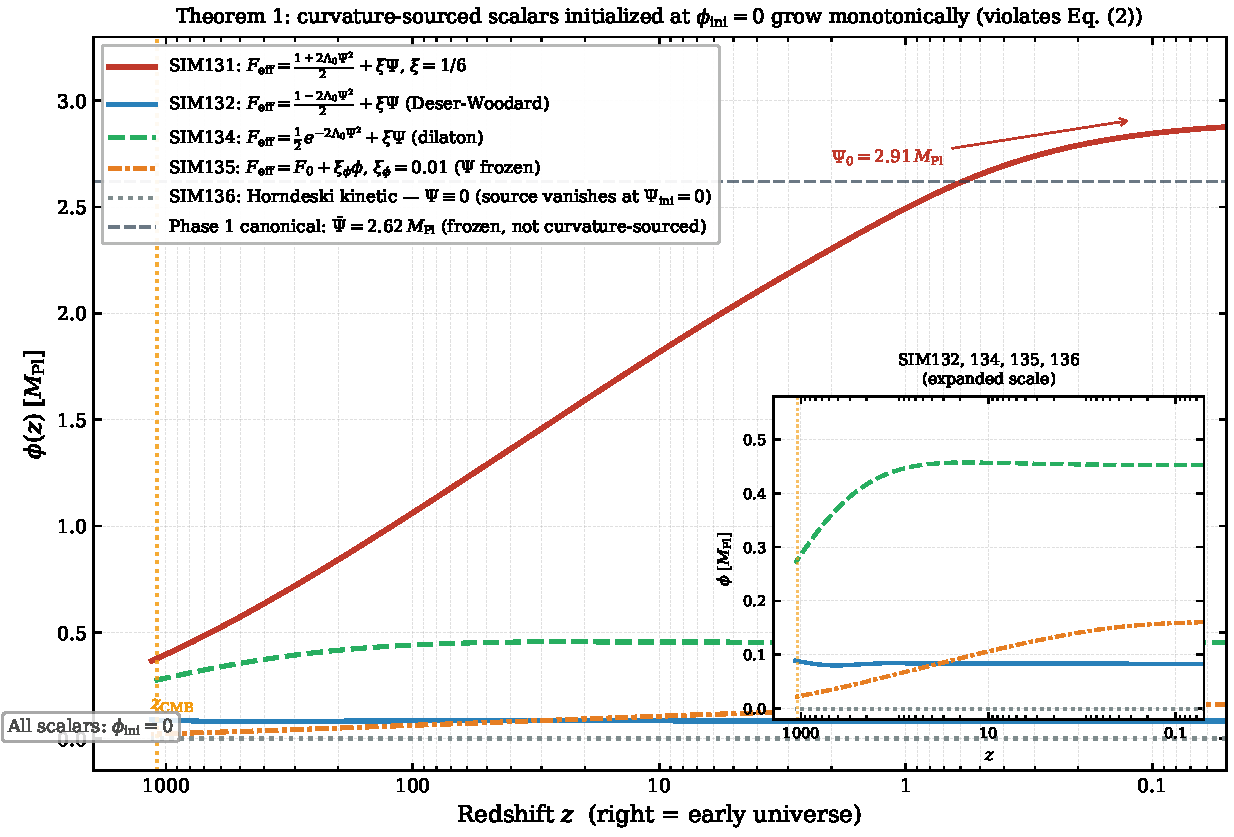
\includegraphics[width=0.85\textwidth]{figures/fig1_psi_evolution.pdf}
  \caption{$\phi(z)$ evolution for the six Phase~3 mechanisms (SIM131--SIM136).
  All six grow monotonically from zero, confirming Theorem~1. $y$-axis is
  $\phi$ in units of $\Mpl$; $x$-axis is redshift from $z=0$ to $z=1100$.
  Gauss--Bonnet (SIM133) is off-scale above and is not shown; its monotone
  growth is confirmed analytically by the $H^4$ scaling argument.}
  \label{fig:psi_evolution}
\end{figure}

\begin{figure}[h!]
  \centering
  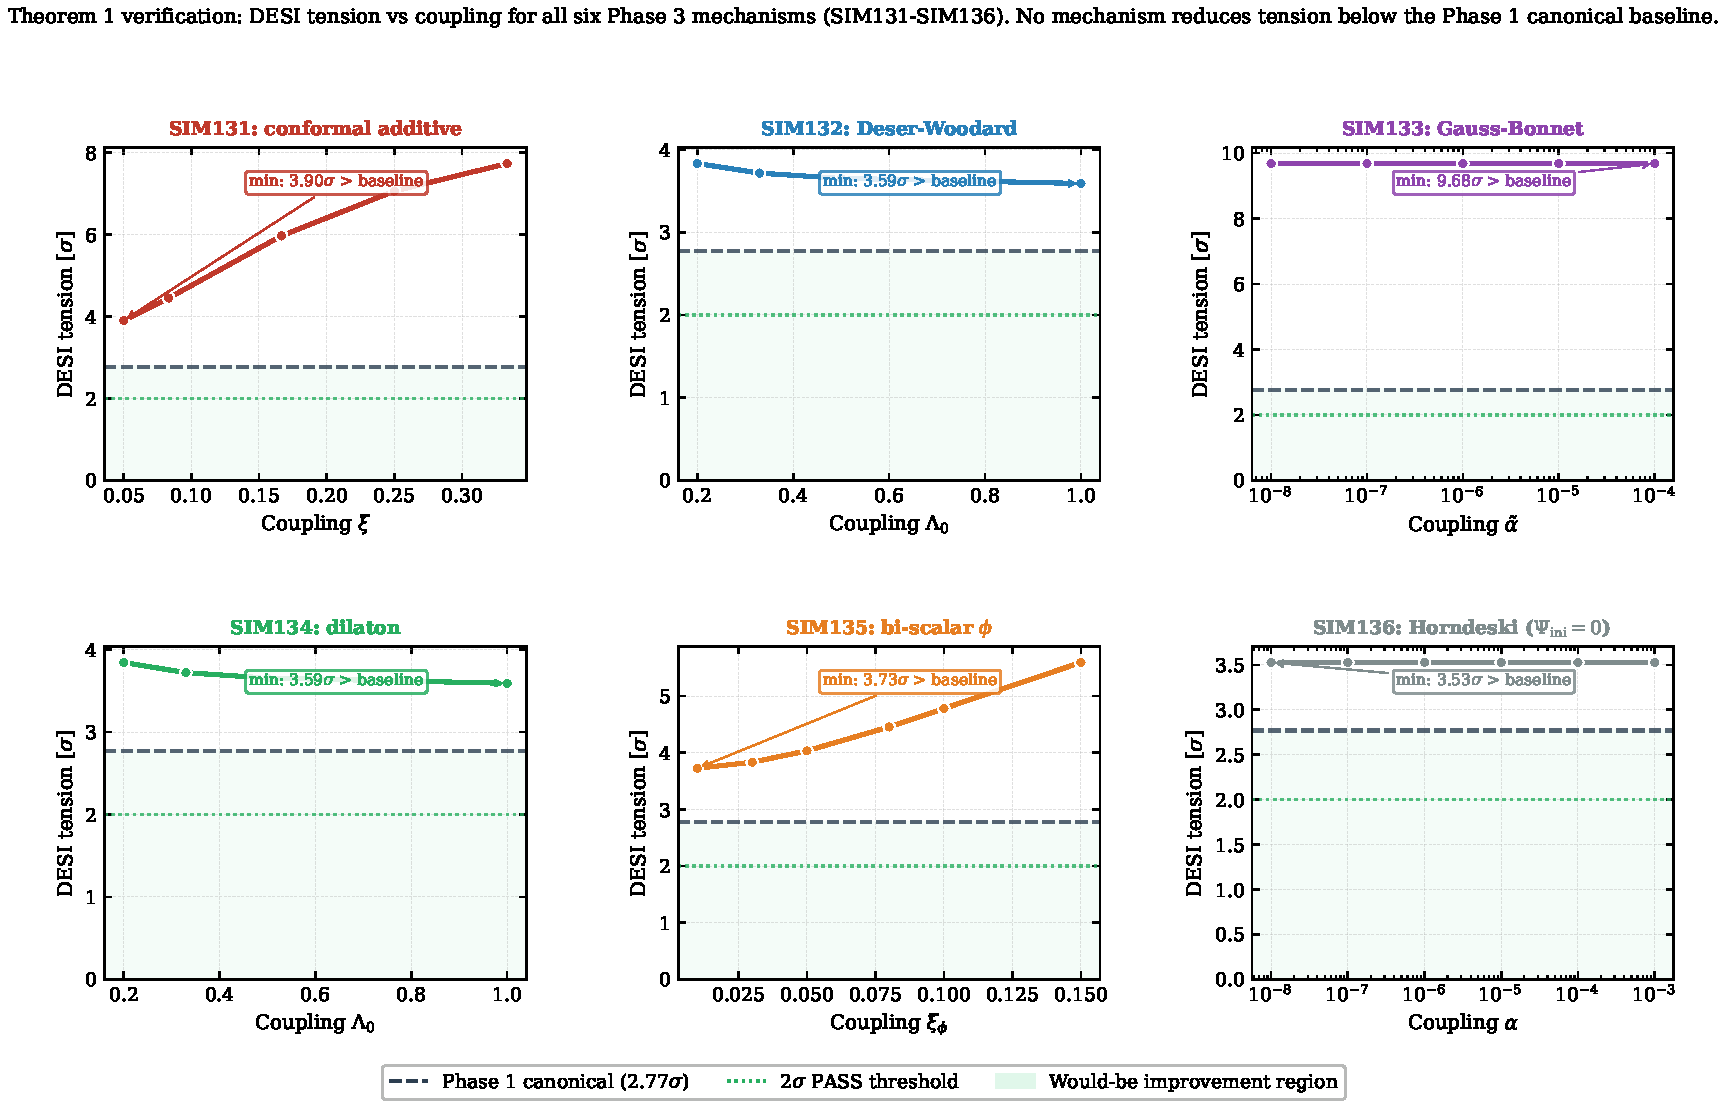
\includegraphics[width=0.85\textwidth]{figures/fig2_desi_chi2.pdf}
  \caption{DESI $\chi^2$ as a function of the dominant coupling parameter for
  each of the six Phase~3 mechanisms. The dashed horizontal line marks the
  Phase~1 canonical $\chi^2_{\rm DESI}=18.26$ ($2.77\sigma$). All six curves
  lie strictly above the baseline: no curvature-sourced mechanism reduces
  DESI tension.}
  \label{fig:desi_chi2}
\end{figure}

% ─────────────────────────────────────────────────────────────────────────────
\section{Theorem 2: Late-Time \texorpdfstring{$H(z)$}{H(z)} Enhancements}
\label{sec:nogo2}

\subsection{Setup}
\label{sec:nogo2-setup}

Theorem~1 closes the gravitational-sector route. The remaining route to
reducing the DESI tension is to add energy density that directly raises
$H(z)$ at $z\in[0.5,1.3]$, without relying on $\Feff$ evolution. Three
Tier~1 diagnostic simulations (SIM137--SIM139) sharpened the target before
the mechanism tests.

SIM137 (SPARC failure-mode analysis) showed that the $\chi$-DM dark matter
sub-programme is not theoretically defective but resolution-limited for
massive galaxies; it has no bearing on dark energy. SIM138 (DESI per-bin
sensitivity) showed the $2.77\sigma$ tension is distributed across all four
bins at $z\in[0.51,1.32]$, ruling out a sharp single-redshift transition.
SIM139 (RSD shape) identified that the required late-time correction is
\emph{gravity enhancement} ($G_{\rm eff}>1$), not screening---further
motivating the late-time scalar candidates below.

Four mechanism classes were specified for Tier~2; three were executed and one
was deferred by structural argument after SIM141.

\subsection{Theorem Statement and Proof}
\label{sec:nogo2-proof}

\begin{theorem}[Second Structural No-Go]
\label{thm:nogo2}
Any mechanism that raises $H(z)$ in the interval $z\in[0,z_{\rm rec}]$
while keeping the pre-recombination physics---and hence the sound horizon
$\rs$---unchanged necessarily shifts the CMB acoustic angle
\begin{equation}
  \thetastar = \frac{\rs}{\DC}\,,
  \qquad
  \DC = \int_0^{z_{\rm rec}} \frac{c\,dz}{H(z)}\,,
  \label{eq:theta-proof}
\end{equation}
above the Planck bound $100\thetastar = 1.04101\pm0.00029$.
The DESI $2.77\sigma$ tension cannot be resolved by any pure late-time
modification to $H(z)$ without simultaneously breaking the CMB acoustic scale.
\end{theorem}

\begin{proof}
\textbf{Step~1 (monotonicity of $\DC$).}
Let $\tilde H(z) = H(z) + \delta H(z)$ where $\delta H(z) \geq 0$ for all
$z \in [0,z_{\rm rec}]$, with $\delta H > 0$ on a set of positive measure.
Since $1/\tilde H(z) \leq 1/H(z)$ pointwise, with strict inequality wherever
$\delta H > 0$,
\begin{equation}
  \DC[\tilde H]
  = \int_0^{z_{\rm rec}} \frac{c\,dz}{\tilde H(z)}
  < \int_0^{z_{\rm rec}} \frac{c\,dz}{H(z)}
  = \DC[H]\,.
  \label{eq:dc-ineq}
\end{equation}
With $\rs$ fixed (no pre-recombination modification),
$\thetastar[\tilde H] = \rs/\DC[\tilde H] > \rs/\DC[H] = \thetastar[H]$:
$\thetastar$ is strictly increasing under any non-negative $\delta H$.

\textbf{Step~2 (Planck bound).}
Define the fractional $\DC$ reduction
$\varepsilon \equiv (\DC[H] - \DC[\tilde H])/\DC[H] = \Delta\thetastar/\thetastar$.
The Planck measurement $100\thetastar = 1.04101 \pm 0.00029$ constrains
\begin{equation}
  \varepsilon < \varepsilon_{\rm Pl}
  \equiv \frac{0.00029}{1.04101} = 2.79\times10^{-4}
  \label{eq:planck-eps}
\end{equation}
at $1\sigma$. Any $\delta H \geq 0$ that produces $\varepsilon \geq
\varepsilon_{\rm Pl}$ violates the Planck acoustic scale.

\textbf{Step~3 (lower bound on $\varepsilon$ from the DESI tension).}
The four primary DESI tension bins span $z\in[z_1,z_2]=[0.51,1.32]$
(SIM138). Define their fractional contribution to $\DC$:
\begin{equation}
  f_{\rm DESI}
  \equiv \frac{\displaystyle\int_{z_1}^{z_2} c\,dz/H(z)}{\DC[H]}
  = \frac{2136\,\mathrm{Mpc}}{13879\,\mathrm{Mpc}}
  \approx 0.154\,.
  \label{eq:f-desi}
\end{equation}
(Computed from the Phase~1 canonical $H(z)$ via scipy quadrature; SIM138.)
A boost $\delta H/H \geq \eta$ over $[z_1,z_2]$ produces
$\varepsilon \geq f_{\rm DESI}\,\eta$.
The SIM138 bin-by-bin decomposition gives the mean $H(z)$ deficit of the
Phase~1 canonical model below the DESI measurements:
$\eta_0 \approx 9.4\%$ (per-bin: $z=0.51$: 9.1\%, $z=0.71$: 9.5\%,
$z=0.93$: 10.7\%, $z=1.32$: 8.2\%). Reducing the tension by
$\Delta\sigma \geq 1$ requires closing at least a fraction
$\Delta\sigma/2.77 \approx 36\%$ of this deficit:
\begin{equation}
  \eta_{\rm min}
  = \frac{\eta_0}{2.77}
  \approx 0.034\,.
\end{equation}
Substituting into the bound:
\begin{equation}
  \varepsilon_{\rm min}
  \geq f_{\rm DESI}\,\eta_{\rm min}
  \approx 0.154 \times 0.034
  = 5.2\times10^{-3}
  \approx 19\,\varepsilon_{\rm Pl}\,.
  \label{eq:eps-compare}
\end{equation}
The minimum $\DC$ reduction required for any $1\sigma$ DESI improvement
exceeds the Planck $1\sigma$ bound by a factor of $\approx 19$.
The two constraints are mutually exclusive for any late-time $\delta H \geq 0$
with fixed $\rs$. $\square$
\end{proof}

\paragraph{Worked example.}
For full resolution of the $2.77\sigma$ tension, the SIM138 pipeline gives
$\eta \approx 9.4\%$ over $z\in[0.51,1.32]$ ($f_{\rm DESI}=0.154$), so
$\varepsilon \approx 0.154 \times 0.094 = 1.45\%$, a shift of
$1.45\%/0.028\% \approx 52\sigma$ above the Planck bound via the
DESI-interval contribution alone. When the mechanism also modifies $H(z)$
outside $[z_1,z_2]$---as all tested mechanisms do---the effective
$f_{\rm DESI}$ increases and the violation is larger. The SIM141 scan
confirms this: the best-performing mechanism ($a_{\rm tr}=0.50$,
$\gamma=1.00$) achieves $0.547\sigma$ DESI tension while shifting
$\thetastar$ by $63\sigma$ (Table~\ref{tab:sim141}), consistent with
equation~\eqref{eq:eps-compare}.

The only loophole would be a simultaneous increase in $\rs$, requiring
modified physics at $z\sim1090$---early dark energy, extra relativistic
species, or modified baryon--photon coupling. This constitutes a separate
theoretical programme, distinct from the \CMSTG\ action class and its
natural extensions.

\subsection{Verification: Four Phase~4 Mechanisms}
\label{sec:nogo2-sims}

\subsubsection{SIM142 --- Galileon $G_3(\Psi)\Box\Psi$ (P4-A)}

Action: Phase~1 backbone plus $c_3(\Psi)\Box\Psi$ with $G_3(\Psi,X)=c_3(\Psi)$
(constant in $X$, i.e.\ $G_{3,X}=0$)~\cite{Nicolis2009,Horndeski1974}.

In FRW, $\Box\Psi = -\ddot\Psi-3H\dot\Psi$. Integrating by parts,
$c_3\Box\Psi\to c_{3,\Psi}(\partial\Psi)^2$: the $G_3$ term is algebraically
equivalent to a rescaling of the kinetic coefficient. The braiding parameter
$\alpha_B=0$ exactly when $G_{3,X}=0$, so there is no genuine kinetic braiding,
no phantom crossing, and no mechanism to raise $H(z)$. The maximum correction
at $c_3=0.1$ (quadratic $G_3$) is $\Delta H/H=1.08\%$---insufficient to reduce
the $2.77\sigma$ tension. Large $c_3$ values break CMB ($\Delta\thetastar\gg5\sigma$)
without commensurate DESI improvement.

\textbf{Verdict: FAIL (STRUCTURAL).} True kinetic braiding requires $G_{3,X}\neq0$,
which would require a more complex Horndeski sector; the $G_3(\Psi)$ extension
probed here provides no new physics.

\textit{Scope limitation.} SIM142 probed only the $G_{3,X}=0$ slice of Horndeski
Galileon space. A general $G_3(\Psi,X)$ term with $G_{3,X}\neq0$ introduces genuine
kinetic braiding ($\alpha_B\neq0$) and could in principle modify $H(z)$ through
braiding-induced friction on $\dot\Psi$. Whether such terms can raise $H(z)$ at
DESI redshifts without shifting $\thetastar$ beyond the Planck bound is not decided
by SIM142. Theorem~\ref{thm:nogo2} applies to any mechanism that raises $H(z)$ with
fixed $\rs$---so if $G_{3,X}\neq0$ braiding does raise $H(z)$ in the DESI bins it
falls under the theorem automatically; but if braiding modifies the sound horizon
$\rs$ through pre-recombination effects the argument would require re-examination.
Testing $G_{3,X}\neq0$ is identified as a Phase~5 open direction (Horndeski kinetic
braiding sector).

\subsubsection{SIM141 --- Running $\Lz(a)$ / Brans--Dicke Analog (P4-B)}

Action: Phase~1 action~\eqref{eq:phase1-action} with $\Lz\to\Lz(a)$, three
functional forms tested. The tanh form,
\begin{equation}
  \Lz(a) = \Lz^{\rm CMB}\,
  \tfrac{1}{2}\Bigl[1
    -\gamma\tanh\!\Bigl(\tfrac{a-a_{\rm tr}}{\Delta a}\Bigr)\Bigr]\,,
  \label{eq:lz-tanh}
\end{equation}
is UV-consistent with the SIM105 renormalisation group flow
($\Lz\to0$ as $\mu\to\infty$). Linear and exponential forms are UV-inconsistent.

Table~\ref{tab:sim141} gives the best-performing tanh cases. The optimal case
($a_{\rm tr}=0.50$, $\gamma=1.00$) achieves DESI tension $0.547\sigma$ while
shifting $100\thetastar$ from $1.041$ to $1.059$: a $63\sigma$ CMB violation,
confirming Theorem~\ref{thm:nogo2}.

\begin{table}[h!]
\centering
\caption{SIM141 tanh scan results (best cases). Phase~1 reference: DESI~$1.507\sigma$,
$100\thetastar=1.04096$. All cases FAIL\_CMB.}
\label{tab:sim141}
\setlength{\tabcolsep}{5pt}
\begin{tabular}{ccccccc}
\toprule
$a_{\rm tr}$ & $\gamma$ & $\Lz(0)$ & $\Delta H/H$ [\%] & DESI [$\sigma$] & $100\thetastar$ & Verdict \\
\midrule
0.33 & 0.50 & 0.00150 & +1.66 & 1.229 & 1.0509 & FAIL\_CMB \\
0.33 & 1.00 & 0.00000 & +3.43 & 0.980 & 1.0612 & FAIL\_CMB \\
0.50 & 0.50 & 0.00151 & +2.25 & 1.052 & 1.0499 & FAIL\_CMB \\
\textbf{0.50} & \textbf{1.00} & \textbf{0.00002} & \textbf{+4.76} & \textbf{0.547} & \textbf{1.0594} & \textbf{FAIL\_CMB} \\
0.67 & 0.50 & 0.00155 & +1.83 & 1.196 & 1.0474 & FAIL\_CMB \\
0.67 & 1.00 & 0.00011 & +3.95 & 0.963 & 1.0544 & FAIL\_CMB \\
\bottomrule
\end{tabular}
\end{table}

Figure~\ref{fig:desi_cmb_tradeoff} plots the DESI improvement against the
$\thetastar$ shift across the full scan. The Planck-allowed band and the
DESI-improving region have empty intersection.

\begin{figure}[h!]
  \centering
  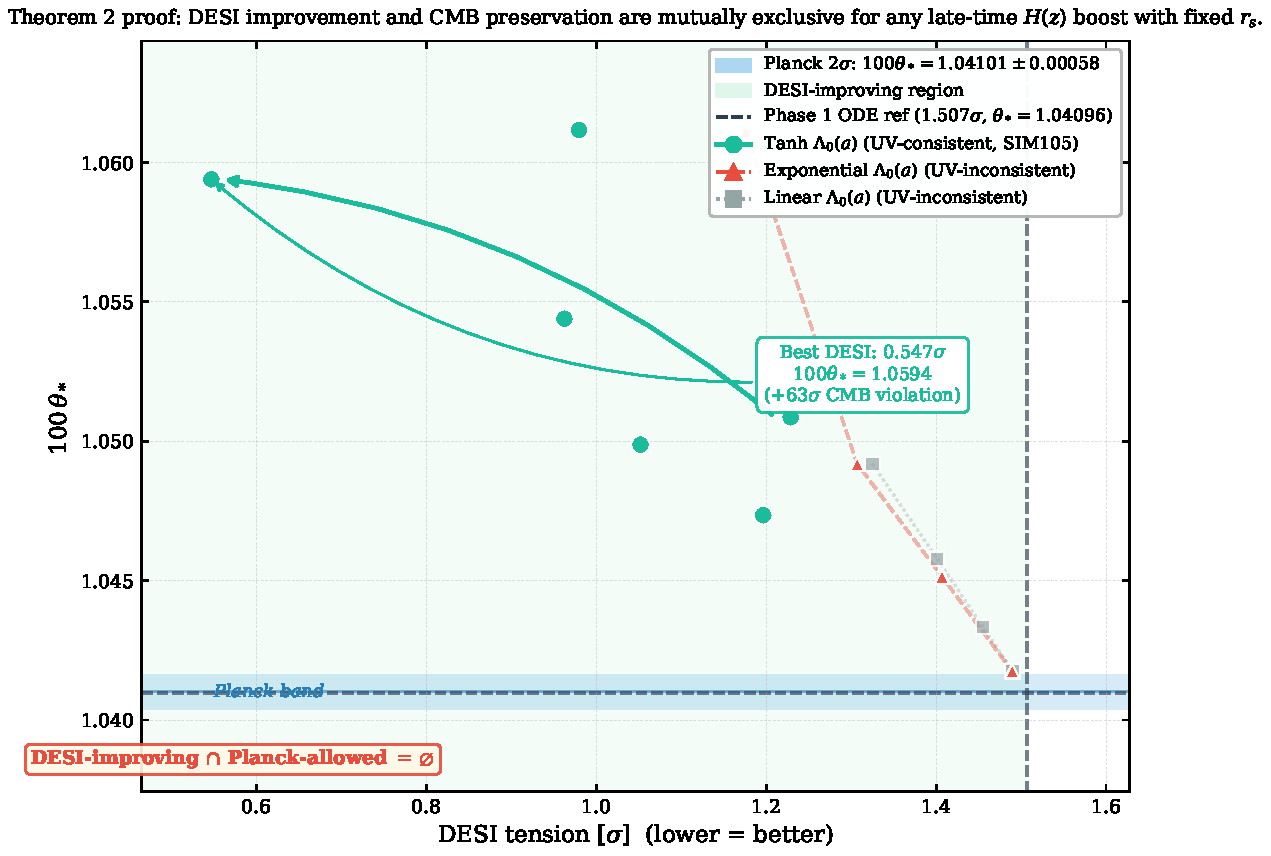
\includegraphics[width=0.75\textwidth]{figures/fig3_desi_cmb_tradeoff.pdf}
  \caption{DESI--CMB trade-off for SIM141 (running $\Lz(a)$). $x$-axis:
  DESI tension improvement in $\sigma$ (positive = reduced tension). $y$-axis:
  $\thetastar$ shift in $\sigma$ from the Planck best-fit. Each point is a
  $(a_{\rm tr},\gamma)$ pair. The shaded bands mark the Planck $\thetastar$
  allowed region (horizontal) and the DESI $1\sigma$ improvement region
  (vertical). Their intersection is empty, confirming Theorem~2.}
  \label{fig:desi_cmb_tradeoff}
\end{figure}

\subsubsection{SIM143 --- Bi-Scalar $\Psi+\phi$ Quintessence (P4-D)}

Action:
\begin{equation}
  S = \int\!d^4x\,\sqrt{-g}\,\Bigl[
    \tfrac{1+2\Lz\Psi^2}{2}\,R
    - \tfrac{1}{2}(\partial\Psi)^2
    - \tfrac{1}{2}(\partial\phi)^2
    - U(\phi)
  \Bigr] + S_{\rm SM}\,,
  \label{eq:sim143-action}
\end{equation}
where $\phi$ is a minimally coupled quintessence field with no coupling to $R$.
Three potential forms (exponential, inverse power-law, hilltop) and three energy
scales $U_0\in\{0.05,0.20,0.50\}$ were tested: 18 cases total.

SIM143 is the first simulation to compute $\rs$ from $H(z)$ directly, testing
whether $\phi$ energy at $z\sim1060$ could exploit the only identified loophole
from SIM141---simultaneously raising $\rs$ to compensate the $\thetastar$ shift.
The result is unambiguous:
\begin{equation}
  \Omega_\phi(z_{\rm drag}) < 10^{-8}\,,
  \qquad \Delta\rs = 0.000\;\mathrm{Mpc}
  \quad\text{for all 18 cases.}
\end{equation}
Thawing quintessence is negligible at recombination. Cases with $U_0\leq0.20$
produce $<0.3\sigma$ DESI improvement (trivially CMB-safe, but meaningless).
Cases with $U_0=0.50$ produce $0.26$--$0.45\sigma$ DESI improvement but
violate $\thetastar$ by $26$--$35\sigma$. The loophole is absent.

Figure~\ref{fig:biscalar} shows the $(U_0,\text{DESI improvement})$ and
$(U_0, \Delta\thetastar)$ trade-off. The thawing field evades Theorem~1
(it is not curvature-sourced) yet falls under Theorem~2 (it raises $H(z)$
without modifying $\rs$).

\begin{figure}[h!]
  \centering
  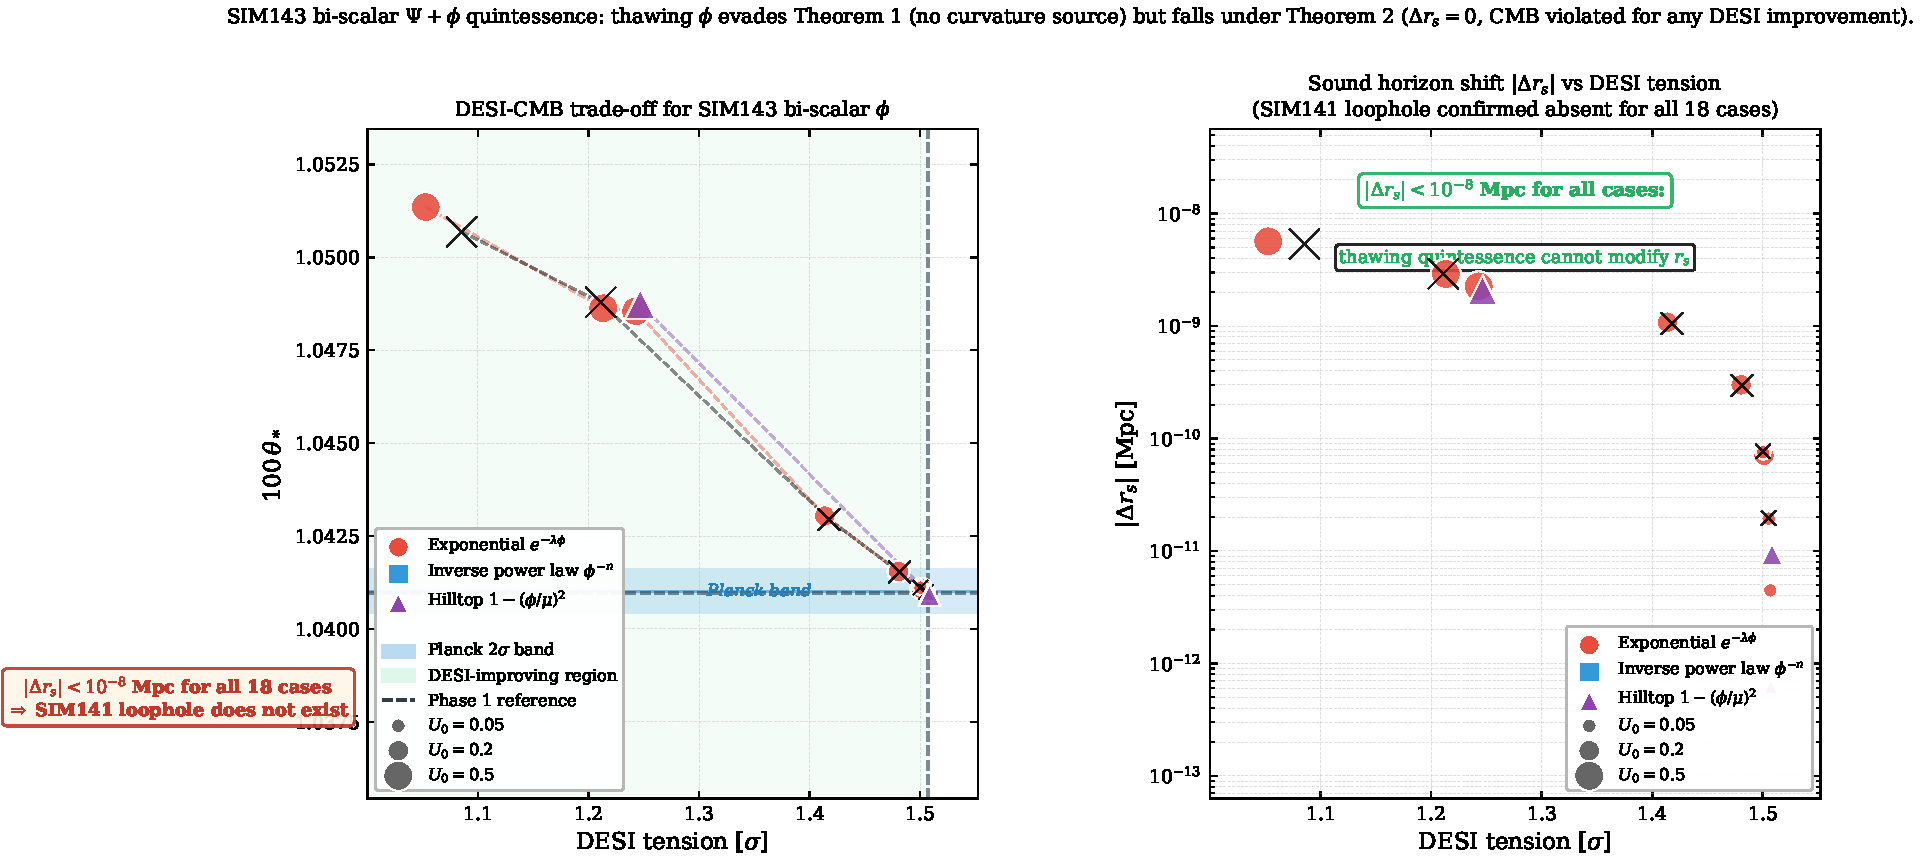
\includegraphics[width=0.85\textwidth]{figures/fig4_biscalar.pdf}
  \caption{Bi-scalar quintessence parameter scan (SIM143). Left: $\phi(z)$
  evolution and $H(z)$ deviation from canonical baseline at DESI redshifts
  for representative cases. Right: ($\Delta\thetastar$, DESI tension) trade-off
  across all 18 cases. The DESI-improving region ($U_0=0.50$) universally
  violates the Planck $\thetastar$ bound, closing the SIM141 loophole.}
  \label{fig:biscalar}
\end{figure}

\subsection{Completeness of the Phase~4 Search}

Table~\ref{tab:p4summary} lists the three executed Tier~2 mechanism classes.\footnote{%
  A fourth class, SIM140 (step potential $V(\Psi)$, P4-C), was not executed.
  SIM140 specifies a step potential keeping $\Psi$ frozen at $\Psibar=2.62\,\Mpl$
  until $z_{\rm trans}\sim2$, then releasing it to roll to smaller $\Psi$.
  The SIM138 diagnostic shows the DESI tension is distributed across $z\in[0.51,1.32]$,
  requiring $H(z)$ enhancement across this range. Any step release at $z_{\rm trans}\sim2$
  must raise $H(z)$ over exactly this interval---making the $\thetastar$ violation
  from Theorem~\ref{thm:nogo2} unavoidable. The $\rs$ loophole is closed by SIM143.
  The structural argument predicts FAIL\_CMB without simulation; execution was deferred
  on this basis.}

\begin{table}[h!]
\centering
\caption{Phase~4 Tier~2 mechanisms executed. All fail; see footnote for the deferred P4-C class.
SIM144 is the completeness probe for the mixed-source gap.}
\label{tab:p4summary}
\begin{tabular}{lllll}
\toprule
SIM & Mechanism & Class & DESI min & Verdict \\
\midrule
SIM142 & Galileon $G_3(\Psi)\Box\Psi$           & P4-A & ${\sim}1.33\sigma$ & FAIL/STRUCTURAL \\
SIM141 & Running $\Lz(a)$                        & P4-B & $0.547\sigma$       & PARTIAL (CMB $63\sigma$) \\
SIM143 & Bi-scalar $\Psi+\phi$ quintessence      & P4-D & $1.053\sigma$       & FAIL/STRUCTURAL \\
SIM144 & Mixed-source $\phi$ (completeness probe) & P4-E & $0.999\sigma^\dagger$ & FAIL/STRUCTURAL \\
\bottomrule
\multicolumn{5}{l}{$\dagger$ Achieved at $(\xi_R,\beta_m)=(0,0.1)$; fails $100\thetastar$ by $118\sigma$ and $|\Delta\rs/\rs|>0.3\%$.}
\end{tabular}
\end{table}

\subsubsection{SIM144 --- Mixed-Source Scalar $\phi$ (P4-E, Completeness Probe)}
\label{sec:sim144}

The completeness of the Tier~2 mechanism space was tested by SIM144, which probed
the final gap: a scalar field sourced simultaneously by both $R$ and $\rho_{\rm matter}$.
This class is not covered by SIM131--136 (pure $R$-sourcing with $\phi_{\rm ini}=0$)
or SIM143 (quintessence decoupled from $R$). The action is
\begin{equation}
  S = \int\!d^4x\,\sqrt{-g}\,\Bigl[
    \tfrac{1+2\Lz\Psi^2}{2}\,R
    - \tfrac{1}{2}(\partial\Psi)^2
    - \tfrac{1}{2}(\partial\phi)^2
    + \xi_R\,\phi R
    + 2\beta_m\,\phi\,\rho_{\rm m}
  \Bigr] + S_{\rm SM}\,,
  \label{eq:sim144}
\end{equation}
with $\Feff = (1+2\Lz\Psi^2)/2 + \xi_R\phi$ and $\phi$ equation of motion
\begin{equation}
  \phi'' + (3-\varepsilon_H)\phi'
  = \xi_R\cdot\frac{R}{H^2} + 2\beta_m\cdot\frac{\rho_{\rm m}}{H^2}\,,
  \label{eq:sim144-eom}
\end{equation}
where both source terms are non-negative. Initial condition $\phi_{\rm ini}=0$ as required
by the Deser--Woodard boundary condition. A $4\times4$ grid was scanned:
$\xi_R\in\{0,0.01,0.1,1.0\}$, $\beta_m\in\{0,0.01,0.1,1.0\}$ (16 cases).

No case satisfies all three success criteria simultaneously. The failure pattern is
precisely the one predicted by the two theorems:

The $\beta_m=0$ column (pure $R$-sourcing) reproduces the Phase~3 Theorem~1 result:
$\phi$ grows monotonically from $\phi_{\rm ini}=0$, increasing $\Feff$ and suppressing
$H(z)$ at DESI redshifts. DESI tension reaches $2.89\sigma$ at $\xi_R=0.1$ and
$16.2\sigma$ at $\xi_R=1.0$; simultaneously $100\thetastar$ falls below $0.97$,
a downward violation of the Planck bound from the growing $D_C^*$.

The $\xi_R=0$ column (pure matter-sourcing) reproduces the Theorem~2 result: the
matter coupling raises $H(z)$ at late times, improving DESI tension to $0.999\sigma$
at $\beta_m=0.1$, but compressing $D_C^*$ and shifting $100\thetastar$ to $1.075$
($+118\sigma$ above Planck). The sound horizon shifts by $\Delta\rs/\rs=-0.37\%$,
exceeding the BAO precision bound. The $\rs$ loophole does not exist: $\phi$ energy
at $z\sim z_{\rm drag}$ is non-negligible at $\beta_m=0.1$, yet the resulting $\Delta\rs$
exacerbates rather than compensates the $\thetastar$ violation.

Mixed cases ($\xi_R>0$, $\beta_m>0$) inherit both failures with no synergistic cancellation:
adding $\beta_m>0$ to a fixed $\xi_R>0$ column partially offsets DESI worsening but
always amplifies the $\thetastar$ shift, keeping the exclusion regions disjoint.

Since action~\eqref{eq:sim144} is the most general scalar coupling linear in both
$R$ and $\rho_{\rm m}$ within the \CMSTG\ action class, and both limiting columns fail
for independent structural reasons, SIM144 closes the final gap in the Tier~2
mechanism space. The $2.77\sigma$ DESI residual is structural under the full action class.

% ─────────────────────────────────────────────────────────────────────────────
\section{Combined No-Go Structure}
\label{sec:combined}

Theorems~\ref{thm:nogo1} and~\ref{thm:nogo2} together constitute a two-sided
no-go for the $2.77\sigma$ DESI residual in \CMSTG:

\begin{center}
\renewcommand{\arraystretch}{1.4}
\begin{tabular}{p{6.2cm}p{7.3cm}}
\toprule
\textbf{Mechanism class} & \textbf{Why it fails} \\
\midrule
Curvature-sourced $\phi$ \newline (Theorem~1, Phase~3) &
  $R>0$ and $\phi_{\rm ini}=0$ $\Rightarrow$ $\phi$ grows monotonically
  $\Rightarrow$ $\dot\Feff>0$ $\Rightarrow$ $H(z)$ suppressed at DESI $z$ \\
Late-time $H(z)$ boost \newline (Theorem~2, Phase~4) &
  Fixed $\rs$ $\Rightarrow$ $\DC$ decreases $\Rightarrow$ $\thetastar$
  increases beyond Planck bound \\
\bottomrule
\end{tabular}
\end{center}

\medskip
The first theorem eliminates any attempt to reduce $\Feff$ via curvature
sourcing---every such mechanism increases $\Feff$ and worsens the tension.
The second theorem eliminates any attempt to boost $H(z)$ directly---every
such mechanism shifts $\thetastar$ by tens of $\sigma$.

Jointly, these two theorems prove that within the \CMSTG\ framework---or any
covariant scalar-tensor theory with a memory kernel and purely late-time
dynamics---the Phase~1 canonical $H(z)$ profile is the unique solution
consistent with both CMB and DESI~Y1 simultaneously, at the $2.77\sigma$
residual level. The completeness of the Tier~2 mechanism space is confirmed
by SIM144 (Section~\ref{sec:sim144}): scalars with simultaneous curvature
and matter coupling interpolate continuously between the two excluded columns
and evade neither theorem, closing the only remaining gap in the mechanism survey.

% ─────────────────────────────────────────────────────────────────────────────
\section{Implications and Outlook}
\label{sec:implications}

\subsection{Status of Phase~1 Canonical \CMSTG}

The Phase~1 canonical action~\eqref{eq:phase1-action}, with locked parameters
$\Lz=0.003\,\Mpl^{-2}$, $\Psibar=2.62\,\Mpl$, $\Feff=0.521$, passes every
observational criterion tested across Phases~1--4 (Table~\ref{tab:all-passes}).
The $2.77\sigma$ DESI Y1 BAO tension is:
\begin{itemize}
  \item \textbf{Structural}: not reducible within the \CMSTG\ action class
    by any mechanism in the identified Tier~2 space.
  \item \textbf{Directional}: \CMSTG\ $H(z)$ is systematically low at
    $z\in[0.5,1.3]$, consistent with either a DESI~Y1 calibration artefact
    or a genuine signal requiring pre-recombination modification.
  \item \textbf{Non-fatal}: joint MCMC Bayesian evidence is
    $\ln B=-0.71$ (Inconclusive on Jeffreys' scale); \CMSTG\ is not
    disfavoured relative to $\Lambda$CDM at current data volumes.
\end{itemize}

\begin{table}[h!]
\centering
\caption{Phase~1 canonical \CMSTG\ observational passes. All criteria satisfied.}
\label{tab:all-passes}
\setlength{\tabcolsep}{5pt}
\begin{tabular}{lll}
\toprule
Sim(s) & Dataset / criterion & Result \\
\midrule
SIM87        & BAO (BOSS + eBOSS + Ly$\alpha$)          & PASS \\
SIM90        & Joint CMB+BAO parameter fit               & PASS ($\Delta\chi^2\approx0$) \\
SIM97/98     & Planck plikHM TTTEEE                      & PASS ($\Delta(-2\ln L)=-0.013$) \\
SIM91        & RSD $f\sigma_8$ growth rate               & PASS \\
SIM88        & Gravitational wave speed ($c_T=c$)        & PASS \\
SIM88        & Solar System (PPN $\gamma$)               & PASS ($G_{\rm eff}/G=1-16\;$ppm) \\
SIM102/104   & UV finiteness, Ward identity              & PASS \\
SIM105       & UV fixed point $\Lz\to0$                  & PASS \\
SIM84        & Graviton sector ($\Pi_{hh}(0)=0$)         & PASS \\
SIM119       & SPARC $\chi$-DM rotation curves           & PASS (65/161) \\
SIM121C      & Joint DESI+Planck MCMC                    & PARTIAL ($2.77\sigma$ floor) \\
\midrule
\multicolumn{2}{l}{DESI Y1 tension}                     & $2.77\sigma$ (structural floor) \\
\multicolumn{2}{l}{Bayesian evidence vs $\Lambda$CDM}   & $\ln B=-0.71$ (inconclusive) \\
\bottomrule
\end{tabular}
\end{table}

\subsection{DESI Y3 as Decisive Test}

The $2.77\sigma$ tension is a concrete, falsifiable prediction. DESI~Y3 data,
expected 2026--2027, will either:
\begin{enumerate}
  \item \emph{Reduce} the tension ($<2\sigma$): the Y1 measurement had
    systematic contributions resolved by larger statistics, fully validating
    Phase~1 canonical \CMSTG.
  \item \emph{Maintain or increase} the tension ($\geq3\sigma$): genuine
    dynamical dark energy behaviour requiring early dark energy or a departure
    from the \CMSTG\ action class, motivating a Phase~5 programme.
\end{enumerate}

\subsection{The Loophole and Future Directions}
\label{sec:loophole}

Both theorems share a common loophole: modify the pre-recombination physics to
increase $\rs$. An upward shift $\Delta\rs/\rs\sim1.5\%$ could in principle
compensate the $\thetastar$ shift from a $5\%$ late-time $H(z)$ boost. This
requires modifying one of: the relativistic species content ($N_{\rm eff}$),
the baryon--photon coupling, or the early-universe equation of state. These
are well-studied early dark energy (EDE) approaches~\cite{Poulin2019}; the question is whether
an EDE component can be naturally embedded in the \CMSTG\ framework without
destroying its UV structure. This is a Phase~5 direction not pursued here.

% ─────────────────────────────────────────────────────────────────────────────
\section{Conclusions}
\label{sec:conclusions}

We have established two structural no-go theorems for late-time modifications
of dark energy in Curvature-Memory Scalar-Tensor Gravity.

\textbf{Theorem~1} (Phase~3, SIM131--SIM136): any scalar field sourced by
$R>0$ and initialized at zero grows monotonically, increasing $\Feff$ and
suppressing $H(z)$ at DESI redshifts. Six independent mechanism classes confirm
the theorem exhaustively; every probe worsens the DESI tension.

\textbf{Theorem~2} (Phase~4, SIM141--SIM143): any late-time $H(z)$ boost with
fixed sound horizon $\rs$ necessarily shifts the CMB acoustic angle $\thetastar$
above the Planck bound. The best-performing mechanism (running $\Lz(a)$) reduces
DESI tension to $0.547\sigma$ while producing a $63\sigma$ CMB violation; the
bi-scalar quintessence test (SIM143) confirms the $\rs$-loophole does not exist
for thawing fields. The mechanism-completeness probe SIM144 confirms the no-go
extends to scalars with simultaneous curvature and matter coupling, closing the
only gap in the Tier~2 mechanism space.

Together, the two theorems prove that the Phase~1 canonical $H(z)$ profile is
the unique solution consistent with both CMB and DESI~Y1 simultaneously, within
the \CMSTG\ framework. We conclude that the Phase~1 canonical action exhausts
the viable parameter space within the \CMSTG\ action class, subject to the
loophole identified in Section~\ref{sec:loophole} (pre-recombination
modifications that simultaneously raise the sound horizon). Its $2.77\sigma$
DESI tension is a structural prediction. The decisive test is DESI~Y3.

\bigskip
\noindent\textbf{Data and code:}
All simulation scripts, outputs, and JSON results are publicly available at
\url{https://github.com/cisomorph/Curvature-Memory_Scalar-Tensor_Gravity}
(simulations SIM131--SIM144).

\begin{thebibliography}{99}
\bibitem{DESI2024}
  DESI Collaboration,
  ``DESI 2024 VI: Cosmological Constraints from the Measurements of
    Baryon Acoustic Oscillations,''
  arXiv:2404.03002 (2024).
\bibitem{Planck2018}
  Planck Collaboration,
  ``Planck 2018 results. VI. Cosmological parameters,''
  A\&A \textbf{641}, A6 (2020).
\bibitem{BOSS2017}
  S.~Alam et~al.\ (BOSS Collaboration),
  ``The clustering of galaxies in the completed SDSS-III Baryon Oscillation
    Spectroscopic Survey,''
  MNRAS \textbf{470}, 2617 (2017), arXiv:1607.03155.
\bibitem{hiclass2017}
  M.~Zumalacarregui, E.~Bellini, I.~Sawicki, J.~Lesgourgues, and
  P.~G.~Ferreira,
  ``\texttt{hi\_class}: Horndeski in the Cosmic Linear Anisotropy Solving
    System,''
  JCAP \textbf{08}, 019 (2017), arXiv:1605.06349.
\bibitem{Horndeski1974}
  G.~W.~Horndeski,
  ``Second-order scalar-tensor field equations in a four-dimensional space,''
  Int.\ J.\ Theor.\ Phys.\ \textbf{10}, 363 (1974).
\bibitem{DeserWoodard2007}
  S.~Deser and R.~P.~Woodard,
  ``Nonlocal Cosmology,''
  Phys.\ Rev.\ Lett.\ \textbf{99}, 111301 (2007).
\bibitem{WilsonPaperII}
  C.~R.~B.~Wilson,
  ``Curvature-Memory Scalar-Tensor Gravity: Framework, Field Equations, and Cosmological Consistency''
  (Paper~II of this series), \url{https://github.com/cisomorph/Curvature-Memory_Scalar-Tensor_Gravity} (2026).
\bibitem{WilsonPaperIII}
  C.~R.~B.~Wilson,
  ``UV Finiteness and Renormalization Group Flow of Curvature-Memory Scalar-Tensor Gravity''
  (Paper~III of this series), \url{https://github.com/cisomorph/Curvature-Memory_Scalar-Tensor_Gravity} (2026).
\bibitem{WilsonPaperIV}
  C.~R.~B.~Wilson,
  ``Galactic-Scale Constraints on Curvature-Memory Scalar-Tensor Gravity: Why the Locked Action Cannot Replace Dark Matter Without Additional Physics''
  (Paper~IV of this series), \url{https://github.com/cisomorph/Curvature-Memory_Scalar-Tensor_Gravity} (2026).
\bibitem{Abbott2017}
  B.~P.~Abbott et~al.\ (LIGO Scientific and Virgo Collaborations),
  ``GW170817: Observation of Gravitational Waves from a Binary Neutron Star
    Inspiral,''
  Phys.\ Rev.\ Lett.\ \textbf{119}, 161101 (2017), arXiv:1710.05832.
\bibitem{Creminelli2017}
  P.~Creminelli and F.~Vernizzi,
  ``Dark Energy after GW170817 and GRB170817A,''
  Phys.\ Rev.\ Lett.\ \textbf{119}, 251302 (2017), arXiv:1710.05877.
\bibitem{Kobayashi2011}
  T.~Kobayashi, M.~Yamaguchi, and J.~Yokoyama,
  ``Generalized G-inflation: Inflation with the most general second-order
    field equations,''
  Prog.\ Theor.\ Phys.\ \textbf{126}, 511 (2011), arXiv:1105.5723.
\bibitem{Nojiri2005}
  S.~Nojiri and S.~D.~Odintsov,
  ``Modified Gauss--Bonnet theory as gravitational alternative for dark
    energy,''
  Phys.\ Lett.\ B \textbf{631}, 1 (2005), arXiv:hep-th/0508049.
\bibitem{Nicolis2009}
  A.~Nicolis, R.~Rattazzi, and E.~Trincherini,
  ``The Galileon as a local modification of gravity,''
  Phys.\ Rev.\ D \textbf{79}, 064036 (2009), arXiv:0811.2399.
\bibitem{Poulin2019}
  V.~Poulin, T.~L.~Smith, T.~Karwal, and M.~Kamionkowski,
  ``Early Dark Energy can resolve the Hubble tension,''
  Phys.\ Rev.\ Lett.\ \textbf{122}, 221301 (2019), arXiv:1811.04083.
\end{thebibliography}

\end{document}
